\documentclass[main.tex]{subfiles}
\begin{document}

\section*{Thu Nov 28 2019}

Now we talk about the \emph{Shapiro time delay of light}.
This will not be on the exam: only the idea of how to sketch the calculation might be asked. 

We want to send signals from A to B, with a massive object very near the geodesic connecting A and B. 

We have the conserved quantities 
%
\begin{align}
  e = \qty(1 - \frac{2GM}{r}) \dv{t}{\lambda  }
\,,
\end{align}
%
and 
%
\begin{align}
  l = r^2 \dv{\varphi }{\lambda  }
\,.
\end{align}

Since the photon path is a null geodesic, we also have the conserved quantity \(u^2= 0\). 
This gives us a relation for \(\dv*{r}{\lambda  }\): so we find 
%
\begin{align}
  \dv{t}{r} = \frac{\dv*{t}{\lambda }}{\dv*{r}{\lambda }}
  \,.
\end{align}
%
Then, if \(d\) is the shortest distance attained by the photon, we have 
%
\begin{align}
  t = 2 \qty(\int_{r_{A}}^{d} \dv{t}{r} \dd{r} + \int_{d}^{r_B} \dv{t}{r} \dd{r})
\,,
\end{align}
%
where we multiply by 2 since we want to compute the time to go from A to B and back again to A, and split the integrals since \(r\) first decreases and then increases. 
Then, we will have \(t = 2\abs{\vec{x}_A - \vec{x}_B} + O(GM)\), and we consider the first order correction. It comes out to be: 
%
\begin{align}
  \Delta t = 4GM \log \qty(\frac{4 r_A r_B}{d^2})
\,,
\end{align}
%
under an assumption of \(d \ll r_{A, B}\). 

Now, we come back to Schwarzschild. 

We want to show that the Schwarzschild horizon looks like a Rindler horizon. We do the coordinate change: \(r = 2GM + \widetilde{r}\) and ignore the angular part: we find 
%
\begin{align}
  \dd{s^2} = - \qty(1 - \frac{2GM}{\widetilde{r} + 2GM}) \dd{t^2} 
+ \qty(1 - \frac{2GM}{\widetilde{r} + 2GM})^{-1} \dd{\widetilde{r}}
\,,
\end{align}
%
but in the regime of \(\widetilde{r}\ll 2GM\) (which is true near the horizon), we find that 
%
\begin{align}
  g_{00} = - \qty(1 - \frac{2GM}{\widetilde{r} + 2GM})
\approx - \qty(1 - \qty(1- \frac{\widetilde{r}}{2GM}))
\,,
\end{align}
%
so we find  
%
\begin{align}
  \dd{s^2} = - \frac{\widetilde{r}}{2GM} \dd{t^2} + \frac{2GM}{\widetilde{r}} \dd{\widetilde{r}^2}
\,.
\end{align}
%
Now we do \((t, \widetilde{r}) \rightarrow (t, \rho )\) with \(\rho = \sqrt{8GM \widetilde{r}}\). The change of coordinates is 
%
\begin{align}
  \dd{\rho } = \sqrt{\frac{8GM}{\widetilde{r}}} \dd{\widetilde{r}}
\,,
\end{align}
%
which means that 
%
\begin{align}
  \dd{s^2} = - \frac{1}{2GM} \frac{\rho^2}{8GM} \dd{t^2} + \dd{\rho^2}
\,,
\end{align}
%
and now we just need to rescale \(t = \eta \times 4GM\): then 
%
\begin{align}
  \dd{s^2} = -\rho^2 \dd{\eta^2 } + \dd{\rho^2} 
\,.
\end{align}

The old coordinates \((t, r, \theta, \varphi )\) are adapted to a constantly accelerating observer in the Schwarzschild geometry; just like the \(\eta, \rho \) coordinates were adapted to a constantly accelerating observer in the Rindler geometry. 
We see this since the Rindler-like coordinates are constant if and only if the Schwarzschild coordinates are constant. 

However, the horizon is a \emph{horizon} and not a \emph{singularity} since there are coordinates which  make it disappear. 
These are very much non-obvious, however somebody has done it and here is the result: Kruskal-Szekeres coordinates: \((t, r) \rightarrow (U, V)\). They have a different form inside and outside the horizon, however the map \emph{is } continuous across it. 

For \(r>2GM\):
%
\begin{align}
  \begin{cases}
      U &= \cosh(\frac{t}{4GM} ) \qty[\frac{r}{2GM} - 1]^{1/2} \exp(\frac{r}{4GM})  \\
      V &= \sinh(\frac{t}{4GM}) \qty[\frac{r}{2GM} - 1]^{\frac{1}{2}} \exp(\frac{r}{4GM})
  \end{cases}
\,,
\end{align}
%
while for \(r< 2GM\): 
%
\begin{align}
  \begin{cases}
      U &= \sinh(\frac{t}{4GM}) \qty[1 - \frac{r}{2GM}]^{\frac{1}{2}} \exp(\frac{r}{4GM}) \\
      V &= \cosh(\frac{t}{4GM}) \qty[1 - \frac{r}{2GM}]^{\frac{1}{2}} \exp(\frac{r}{4GM}) 
  \end{cases}
\,.
\end{align}

There is no continuity in \(t\), but that is to be expected. We show continuity (and, more importantly, differentiability) in \(r\): 
%
\begin{align}
  U^2 - V^2 = \qty[\frac{r}{2GM}- 1] \exp(\frac{r}{2GM})
\,
\end{align}
%
inside the horizon, but outside of it we have the opposite expression in square brackets: however the hyperbolic sine and cosine are swapped, so we have the same expression. 

[plot of \(U^2- V^2\): it is 0 at \(R = 1\)]

From this expression, we can invert \(r ( U, V)\). 

The line element is given by 
%
\begin{align}
  \dd{s^2} = \frac{32G^3M^3}{r} \exp(-\frac{r}{2GM})
  \qty(- \dd{V^2} + \dd{U^2}) + r^2 \dd{\Omega^2}
\,,
\end{align}
%
where by \(r\) we mean \(r(U,V) = r(U^2-V^2)\), just a shortcut for writing.

Everything is regular except for \(r=0\). 

Now, we discuss \emph{Kruskal diagrams}: the spacetime description in the \(U, V\) coordinates. 

We plot null geodesics in the 2D plane \(U, V\). 
Since \(\dd{s^2} \propto - \dd{U^2} + \dd{V^2}\) and everything multiplying it is positive, then light moves with \( \dv*{V}{U} = \pm 1\). 

Outside the horizon, we have the relations: \(U^2-V^2>0\), and \(U>0\). 

This defines something that looks like a light cone, going rightward from the origin. 

Inside the horizon, we have \(V>0\) and \(V^2-U^2>0\). 

The singularity is \(r=0\) which implies \(U^2- V^2 = -1\), or \(V = \pm \sqrt{1 + U^2}\). 
``It's a parabola with a square root'' 

The regions above and below these hyperbolas have \(r<0\), so they do not exist. 

One might think that the horizon is \(U = V = 0\) by substituting in, but actually it is the whole of \(U = V\) for infinite time \(t\), however this is not a physical problem, it is a problem with the coordinate \(t\) being a bad one. 

Observers moving with constant acceleration (stationary \(r\) in Schwarzschild, only moving throught \(t\)) are hyperbolas, like in Rindler. Lines of constant time instead have constant 
%
\begin{align}
  \frac{V}{U} = \tanh(\frac{t}{4GM})
\,.
\end{align}

Inside the horizon, instead, 
 %
 \begin{align}
   \frac{U}{V} = \tanh(\frac{t}{4GM})
 \,:
 \end{align}
 %
now all the constant-\(t\) lines get to the singularity. 

What about the regions 3 and 4? Light can come from them, through \(t = - \infty\). 

The lower bit of the singularity is called a \emph{white hole}. 

Regions I and IV are mathematically ``connected'', but physically disconnected: no light can travel between them. 

Now: consider a spacetime at fixed time coordinate \(V\), in ``God mode''. 
First, consider \(V \equiv V_0 < 0\): we start in region IV, cross the horizon, reach the white hole, than exit it and move into region I: these two regions (before \& after the WH) are completely disconnected.   


If we restore the coordinate \(\theta \) and draw the space in \(r, \theta \) coordinates as \(U\) changes, then we get something which looks like a wormhole. 

\begin{figure}[ht]
  \centering
  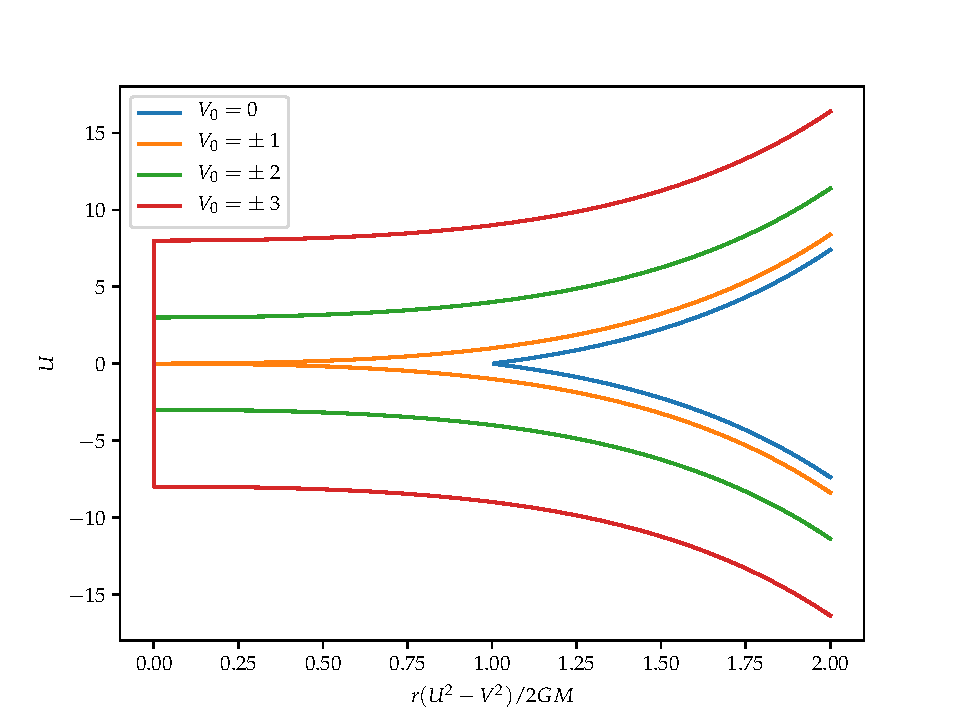
\includegraphics[width=0.7\textwidth]{figures/kruskal_constant_V.pdf}
  \caption{Kruskal \(U\) in terms of Schwarzschild \(r\) at constant \(V\).}
  \label{fig:kruskal-constant-V}
\end{figure}

Every point of this is \((V_0, U_0 , \theta_0 ,  \varphi  )\) with varying \(\varphi \) : a circle.  

\end{document}